\documentclass[nooutcomes,handout]{ximera}
%% handout
%% space
%% newpage
%% numbers
%% nooutcomes

%I added the commands here so that I would't have to keep looking them up
%\newcommand{\RR}{\mathbb R}
%\renewcommand{\d}{\,d}
%\newcommand{\dd}[2][]{\frac{d #1}{d #2}}
%\renewcommand{\l}{\ell}
%\newcommand{\ddx}{\frac{d}{dx}}
%\everymath{\displaystyle}
%\newcommand{\dfn}{\textbf}
%\newcommand{\eval}[1]{\bigg[ #1 \bigg]}

\usepackage{fullpage}
\newcommand{\RR}{\mathbb R}
\renewcommand{\d}{\,d}
\newcommand{\dd}[2][]{\frac{d #1}{d #2}}
\renewcommand{\l}{\ell}
\newcommand{\ddx}{\frac{d}{dx}}
\newcommand{\dfn}{\textbf}
\newcommand{\eval}[1]{\bigg[ #1 \bigg]}

\usepackage{multicol}

\renewenvironment{freeResponse}{
\ifhandout\setbox0\vbox\bgroup\else
\begin{trivlist}\item[\hskip \labelsep\bfseries Solution:\hspace{2ex}]
\fi}
{\ifhandout\egroup\else
\end{trivlist}
\fi} %% we can turn off input when making a master document

\title{3.8: Implicit Differentiation}  

\begin{document}
\begin{abstract}		\end{abstract}
\maketitle

%problem1
\begin{problem}
On the graph below, sketch the tangent lines at $x=0$.  Then, explain why both the $x$-coordinate and the $y$-coordinate are generally needed to find the slope of the tangent line at a point on the graph of an equation of the form $F(x,y)=0$
\begin{image}

\includegraphics[scale=.2]{figure1.png}
\end{image}


	\begin{freeResponse}
		Given the equation $F(x,y)=0$, its graph may not pass the ``vertical line test".  As illustrated in the figure below, fixing a value for $x$ (in this case $x=0$) will not typically specify a unique point on the graph because there may be more than one corresponding $y$-value.  That is why you need to specify both the $x$ and the $y$ coordinate, to make sure that you are giving the coordinates for a unique point on the graph.  In this case, there are two tangent lines to the curve at $x=0$.  One passes through the point $(0,1)$ and the other through $(0,-1)$.
	\begin{image}
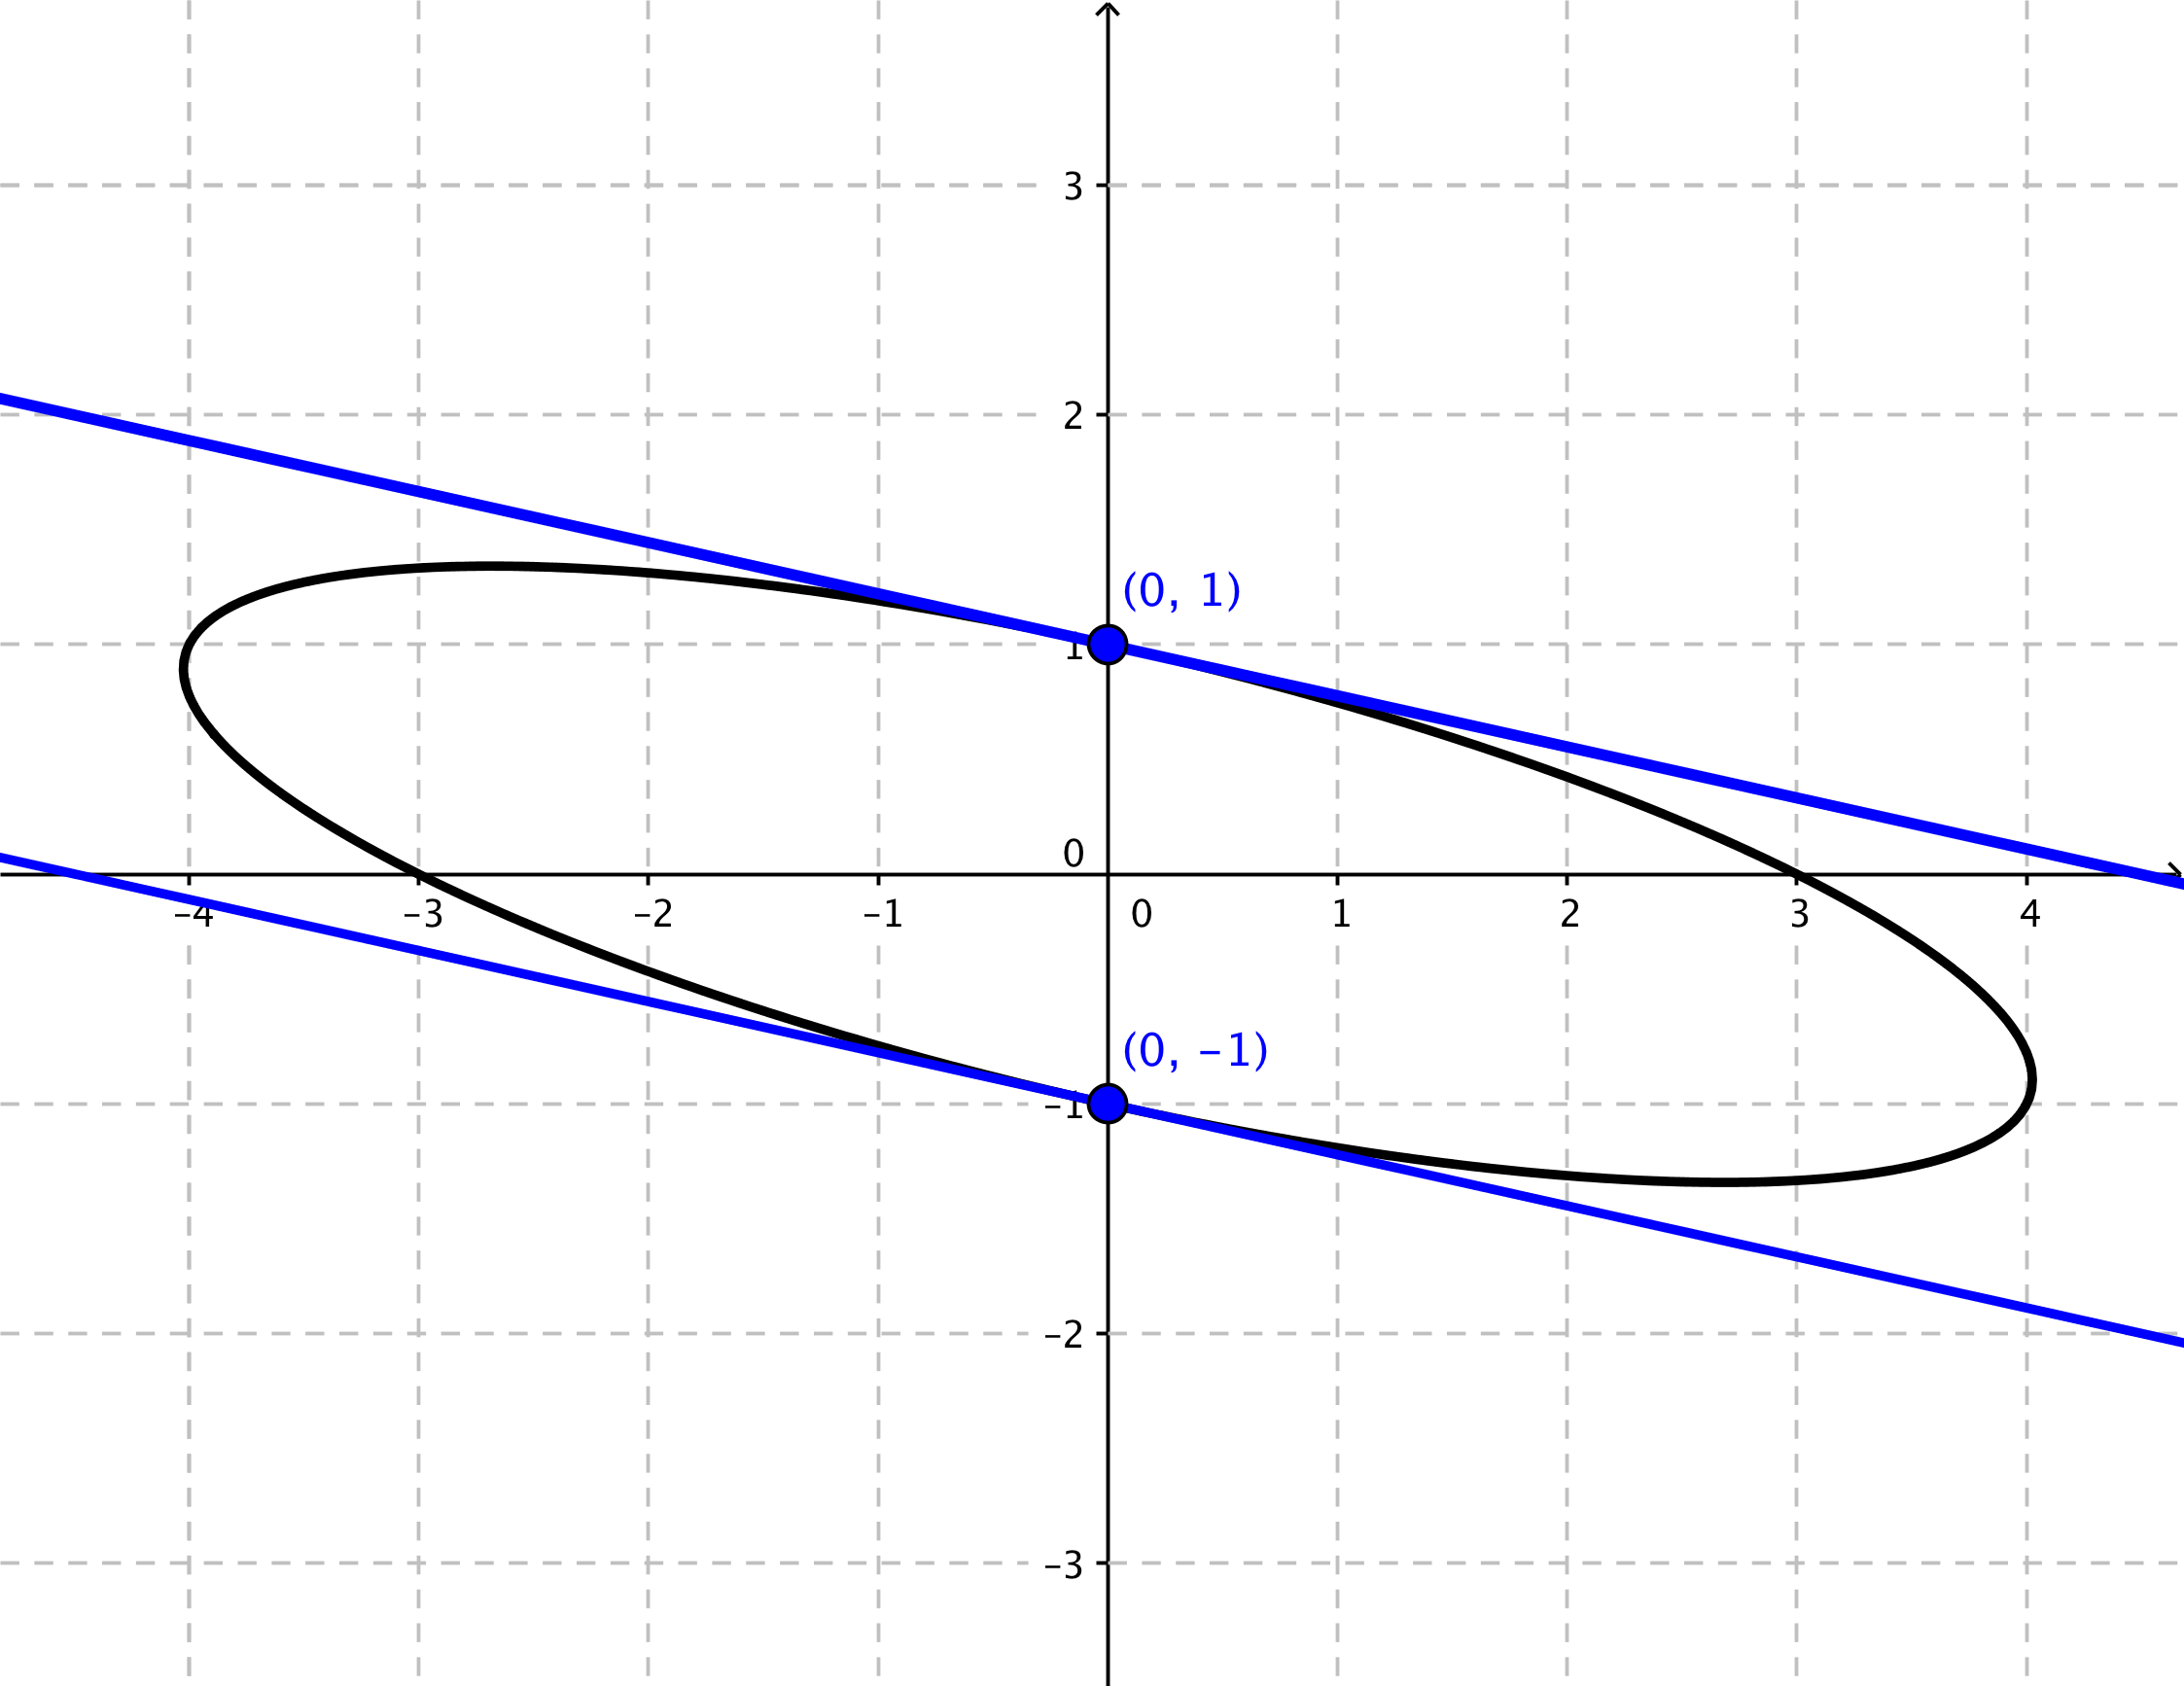
\includegraphics[scale=.5]{figure2.png}
\end{image}		


	\end{freeResponse}	
\end{problem}




%problem2
\begin{problem}
Consider the equation $x^2 + 4xy + 9y^2 = 9$.  Note: This equation is equivalent to $x^2 + 4xy + 9y^2 - 9=0$.  Therefore it has a form $F(x,y)=0$

\begin{image}

\includegraphics[scale=.2]{figure1.png}
\end{image}

	\begin{enumerate}
	
	%part a
	\item  Find $\dd[y]{x}$.
		\begin{freeResponse}
		$$ \ddx(x^2 + 4xy + 9y^2) = \ddx(9) $$
		$$ 2x + \left(4y + 4x \dd[y]{x} \right) + 18 y \dd[y]{x} = 0 $$
		$$ 4x \dd[y]{x} + 18y \dd[y]{x} = -2x - 4y $$
		$$ (4x+18y) \dd[y]{x} = -2x-4y $$
		$$ \dd[y]{x} = \frac{-2x-4y}{4x+18y} $$
		provided that $4x+18y \neq 0$.
		\end{freeResponse}
		
		
		
%part b
	\item  Find the equation(s) of the tangent line(s) when $x=0$.  Draw the tangent line(s) on the above picture.
		\begin{freeResponse}
		Plugging into the original equation, we see that when $x=0$ we have that 
		$$ 0^2 + 4(0)y + 9y^2 = 9 \qquad \Longrightarrow \qquad y^2 = 1 \qquad \Longrightarrow \qquad y = \pm 1 $$
		
		Then,
		$$\eval{\dd[y]{x}}_{(0,1)} = \frac{-4}{18} = -\frac{2}{9}$$
		$$\eval{\dd[y]{x}}_{(0,-1)} = \frac{4}{-18} = -\frac{2}{9} $$
		
		So there are two tangent lines to the graph of the given equation when $x=0$.  The two points are $(0,1)$ and $(0,-1)$, and the tangent lines at both points have slope $-\frac{2}{9}$.  Thus, the equations of the two tangent lines are
		$$ y - 1 = -\frac{2}{9}(x-0)  \qquad \Longrightarrow \qquad y = -\frac{2}{9}x + 1 $$
		$$ y + 1 = -\frac{2}{9}(x-0) \qquad \Longrightarrow \qquad y = -\frac{2}{9}x - 1 $$
\begin{image}
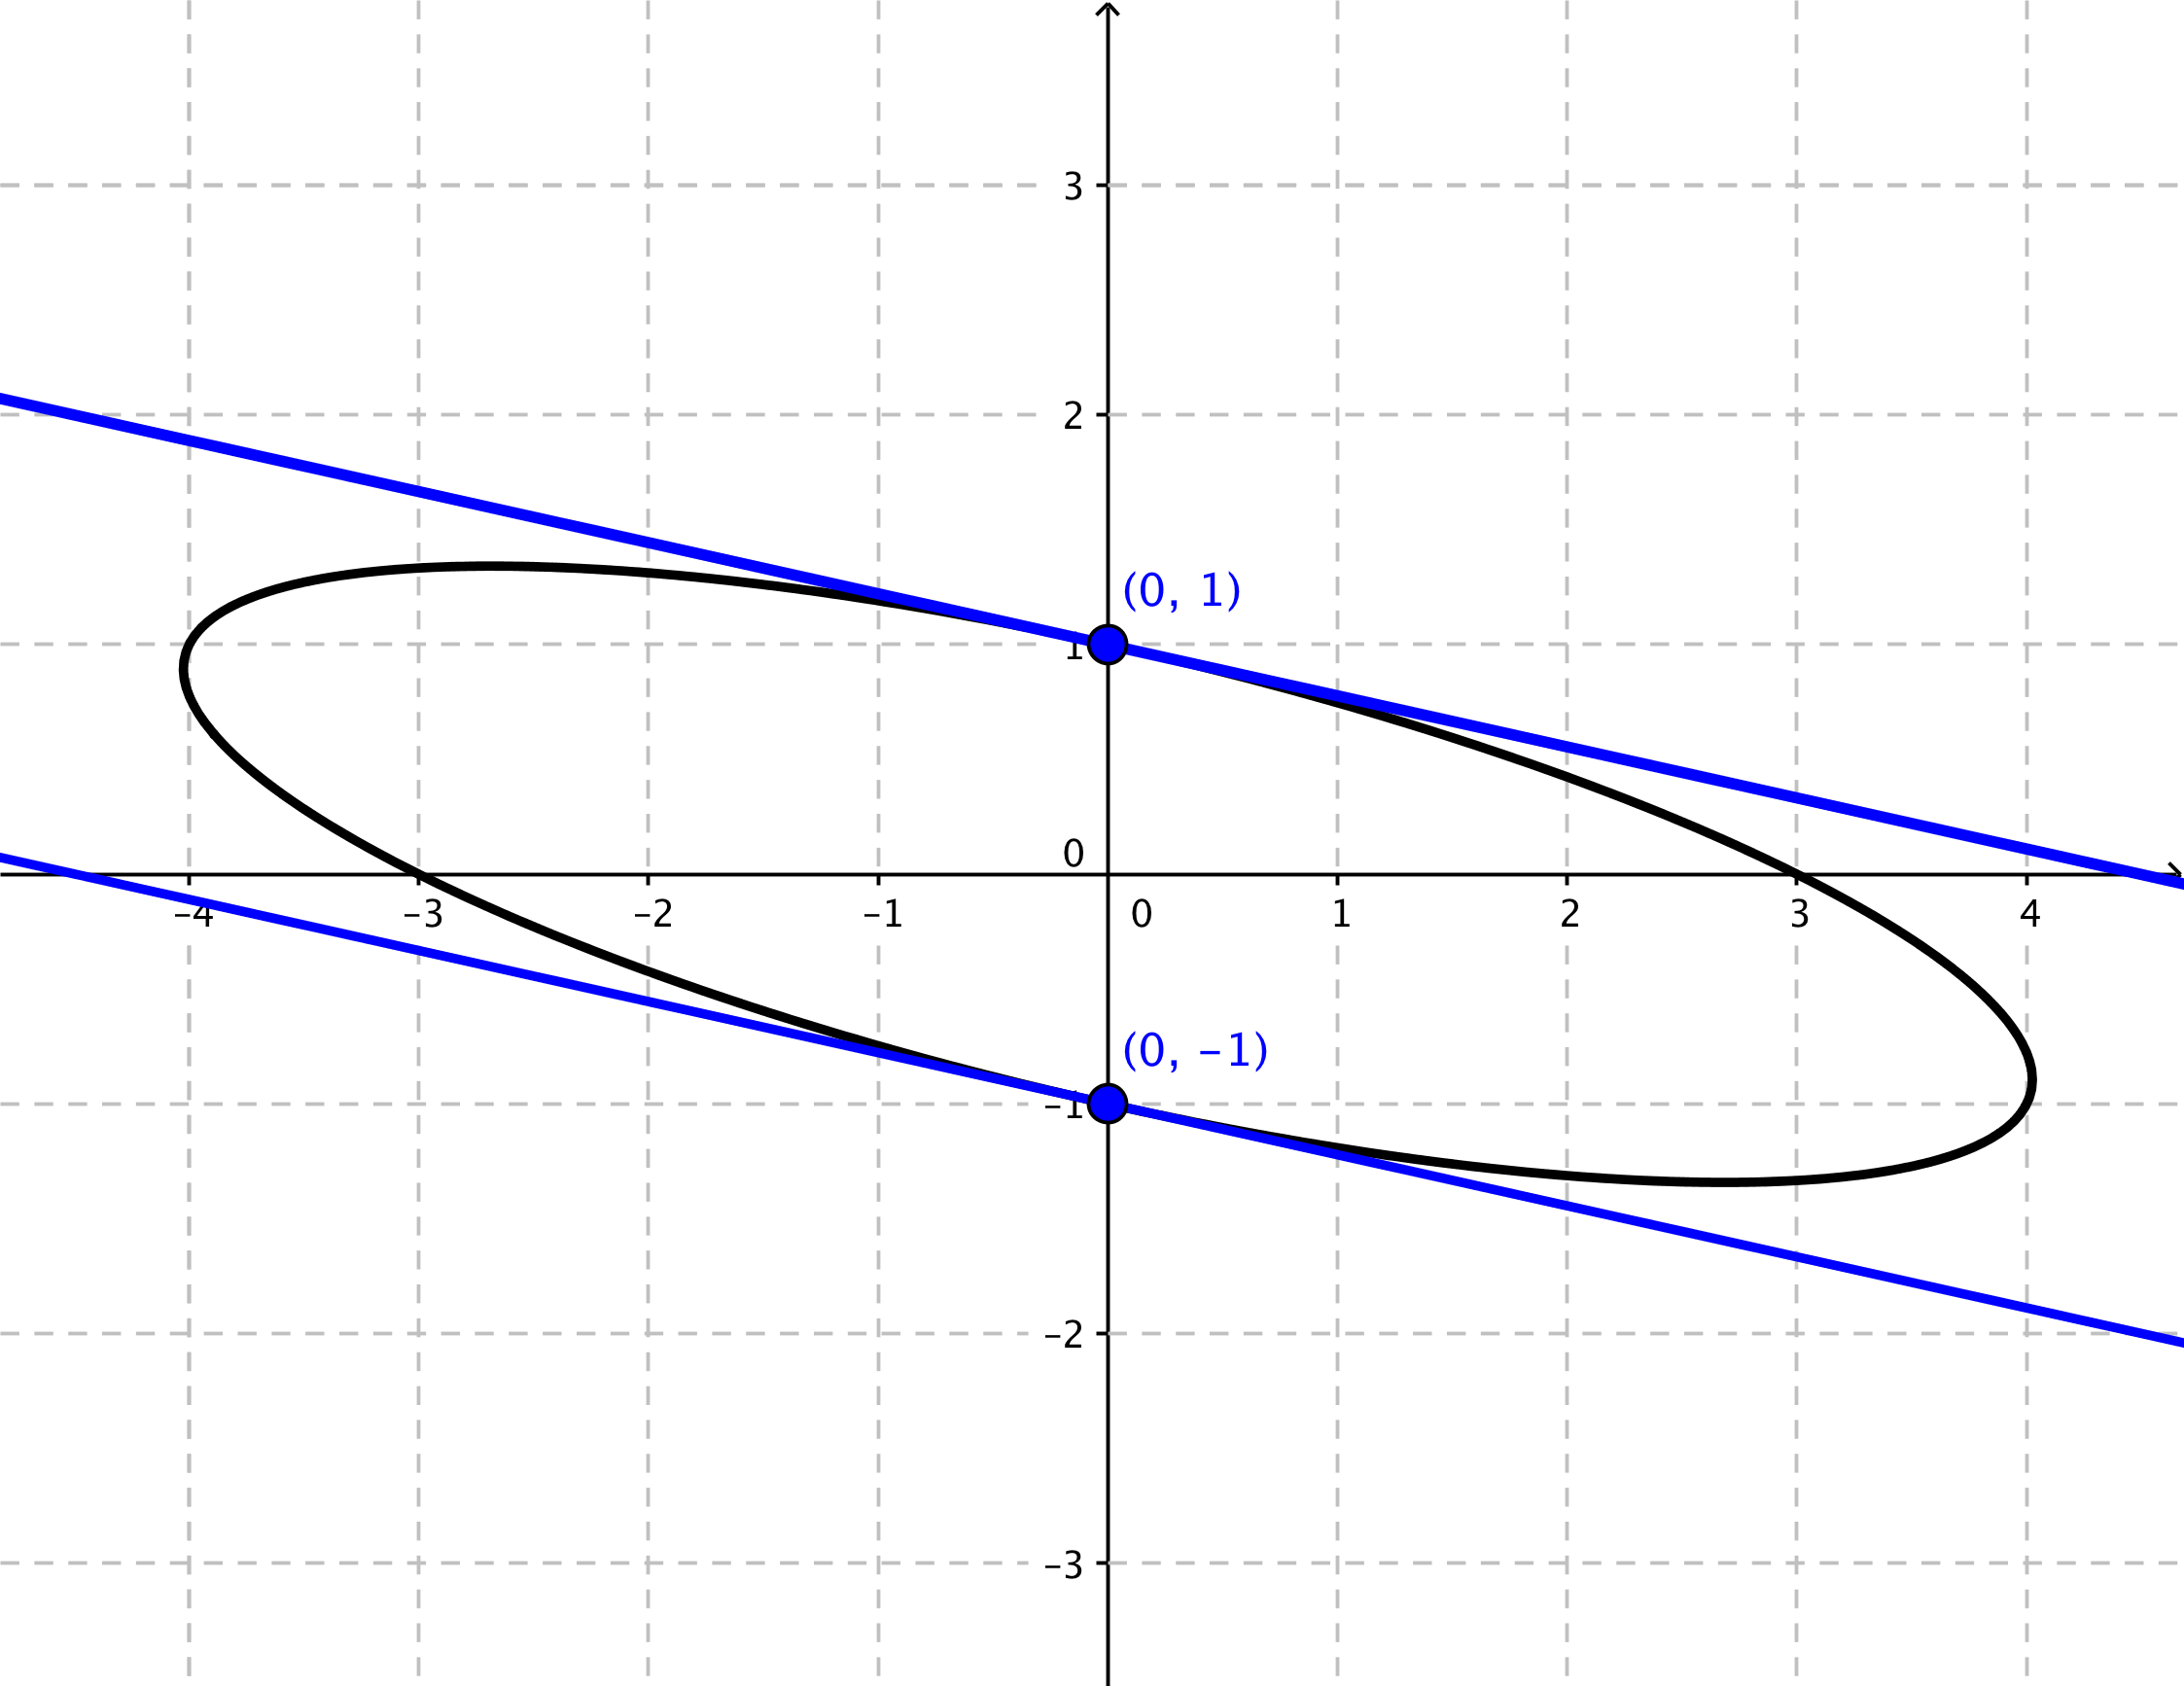
\includegraphics[scale=.6]{figure2.png}
\end{image}		
		
		\end{freeResponse}
		
		
		
%part c
	\item  Find the point(s) where the tangent line is horizontal.  Draw the point(s) and line(s) on the above picture.
		\begin{freeResponse}
		A line is horizontal if and only if its slope is 0.  So we are looking for the points $(x_0,y_0)$ such that $\eval{\dd[y]{x}}_{(x_0,y_0)} = 0$.  So we solve:
		$$ \frac{-2x-4y}{4x+18y} = 0\qquad \Longrightarrow \qquad -2x - 4y = 0 \qquad \Longrightarrow \qquad x=-2y$$
		
		But we also need the point to lie on the the given curve.  So, letting $x=-2y$, we solve:
		$$x^2 + 4xy + 9y^2 = 9 $$
		$$ (-2y)^2 + 4(-2y)y + 9y^2 = 9 $$
		$$ 4y^2 - 8y^2 + 9y^2 = 9 $$
		$$ 5y^2 = 9 $$
		$$ y^2 = \frac{9}{5} $$
		$$ y = \pm \frac{3}{\sqrt{5}} $$
		
		So there exists two solutions to the given equation where the tangent line to the graph has 0 slope.  Those two points are $\left( -\frac{6}{\sqrt{5}}, \frac{3}{\sqrt{5}} \right)$ and $\left( \frac{6}{\sqrt{5}}, - \frac{3}{\sqrt{5}} \right)$.
		
		\begin{image}
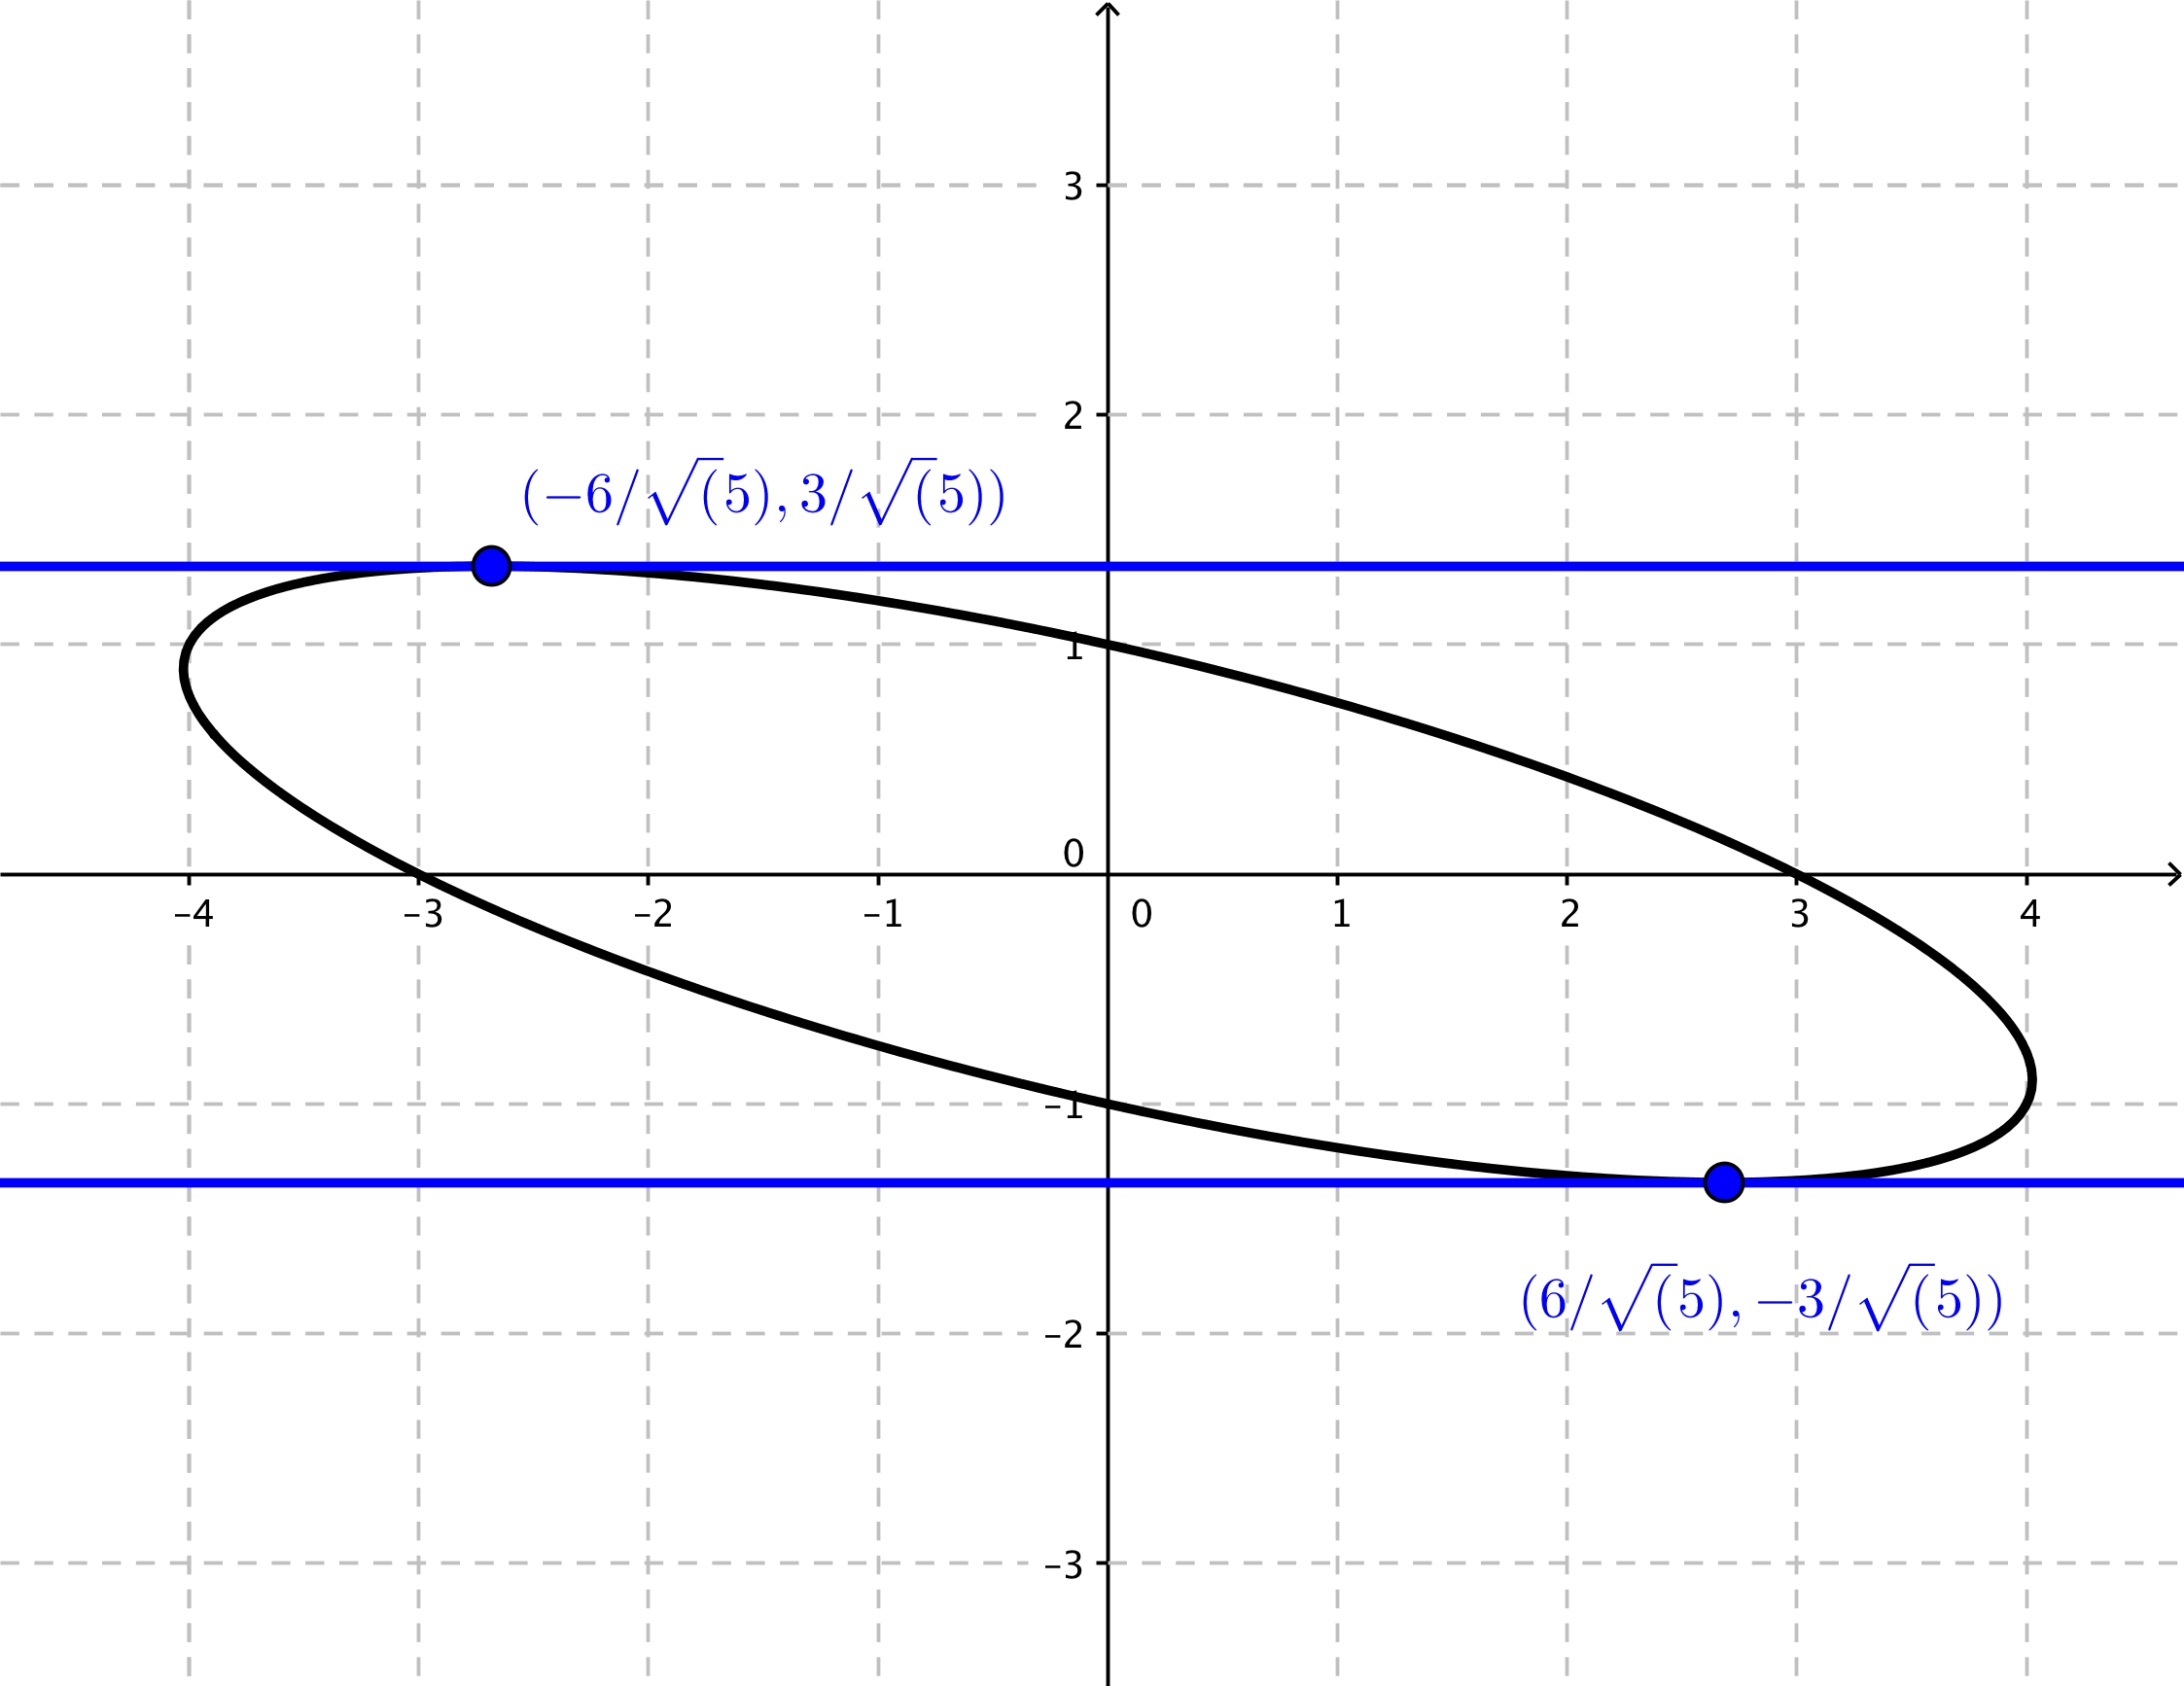
\includegraphics[scale=.6]{figure3.png}
\end{image}		
		
		\end{freeResponse}
		
		
		
	\end{enumerate}
			
			
	
\end{problem}

%problem3
\begin{problem}  A part of the curve with equation $\cos(\pi x y) + x + y = 1$ is sketched below.

  \begin{image}
    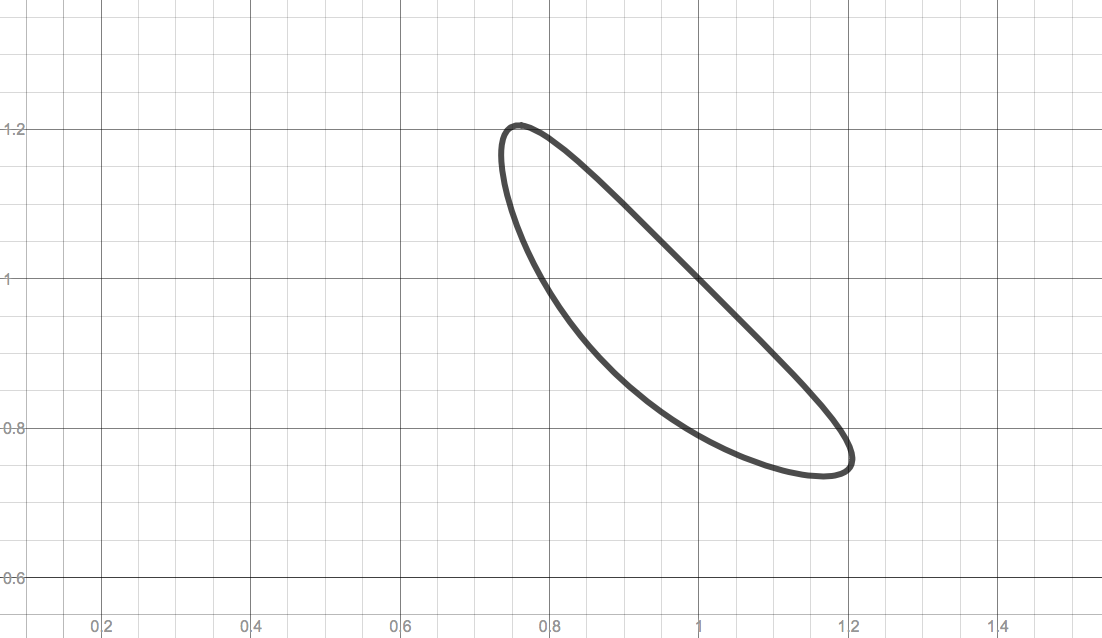
\includegraphics[scale = 0.3]{figure4.png}
  \end{image}
  \begin{enumerate}
    \item
      Use the implicit differentiation to find the derivative $dy/dx$.
      \begin{freeResponse}
        Implicitly differentiate equation:
        \begin{align*}
          \ddx( \cos(\pi x y) + x + y) = \ddx(1) &\implies -\sin(\pi x y)\cdot(\pi y + \pi x \dd[y]{x}) + 1 + \dd[y]{x} = 0 
        \end{align*}

        Solve for $\dd[y]{x}$:
        \begin{align*}
          -\sin(\pi x y)\cdot(\pi y + \pi x \dd[y]{x}) + 1 + \dd[y]{x} = 0 &\implies -\pi y \sin(\pi x y) - \pi x \dd[y]{x} \sin(\pi x y) + 1 + \dd[y]{x} = 0 \\
          &\implies  \bigl(1 - \pi x \sin(\pi x y)\bigr)\dd[y]{x} = \pi y \sin(\pi x y) - 1 \\
          &\implies \dd[y]{x} = \frac{\pi y \sin(\pi x y) - 1}{1 - \pi x \sin(\pi x y)} \hspace{2em} \mbox{if $1 - \pi x \sin(\pi x y) \ne 0$}\\
        \end{align*}
      \end{freeResponse}

    \item
      Consider the point $(1, 1)$.
      Show (algebraically) that this point lies on the curve.
      \begin{freeResponse}
        $(1, 1)$ lies on this curve:
        \begin{align*}
          \cos(\pi \cdot 1 \cdot 1) + 1 + 1 &= \cos(\pi) + 2\\
          &= -1 + 2 = 1
        \end{align*}
      \end{freeResponse}

    \item
      Find the equation of the line tangent to the curve at $(1,1)$.
      Draw this line in the figure above.
      \begin{freeResponse}
        Slope of tangent line:
        \begin{align*}
          \eval{\dd[y]{x}}_{(1,1)} &= \frac{\pi \cdot 1 \cdot\sin(\pi 1 \cdot 1) - 1}{1 - \pi \cdot 1 \cdot \sin(\pi 1 \cdot 1)} \\
          &= \frac{\pi\sin(\pi) - 1}{1 - \pi \sin(\pi)}\\
          &= \frac{-1}{1} = -1
        \end{align*}

        Equation of tangent line:
        \begin{align*}
          y - 1 = -1(x - 1) &\implies y = -x + 2
        \end{align*}

        Graph of tangent line:
        \begin{image}
          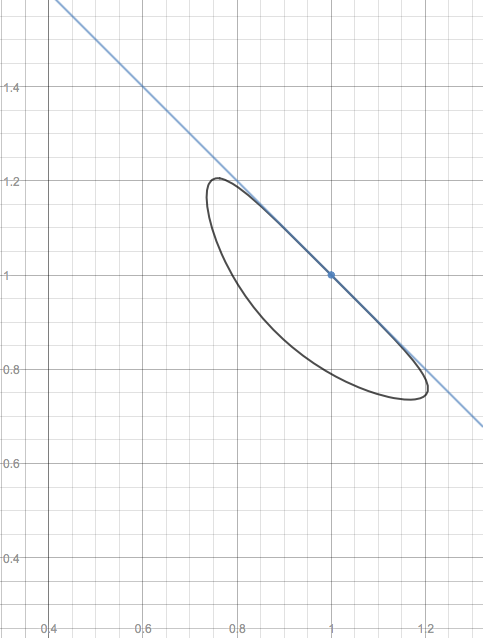
\includegraphics[scale = 0.5]{figure5.png}
        \end{image}
      \end{freeResponse}

  \end{enumerate}
\end{problem}




%problem 4
\begin{problem}
  For each of the curves given by the following equations, find a formula for the slope of the tangent line at a point $(x, y)$.

	\begin{enumerate}
	
	%part a
	\item  $e^{x^2 y^3} - 5x + 7y = 36$
			\begin{freeResponse}
			$$ e^{x^2 y^3} \left( 2xy^3 + x^2 (3y^2)\dd[y]{x} \right) - 5 + 7\dd[y]{x} = 0 $$
			$$ 2xy^3 e^{x^2y^3} + 3x^2y^2e^{x^2y^3}\dd[y]{x} - 5 + 7\dd[y]{x} = 0 $$
			$$ 3x^2y^2e^{x^2y^3}\dd[y]{x} + 7\dd[y]{x} = -2xy^3 e^{x^2y^3} + 5 $$
			$$ \left( 3x^2y^2e^{x^2y^3} + 7 \right) \dd[y]{x} = -2xy^3 e^{x^2y^3} + 5 $$
			$$  \dd[y]{x} = \frac{-2xy^3 e^{x^2y^3} + 5}{3x^2 y^2 e^{x^2y^3} + 7} $$
			\end{freeResponse}
			
			
			
	%part b
	\item  $7 = 22 \tan(y) + \frac{4}{x} - \frac{7}{y}$
			\begin{freeResponse}
			$$ 0 = 22 \sec^2 (y) \dd[y]{x} - \frac{4}{x^2} + \frac{7}{y^2} \dd[y]{x} $$
			$$ 22 \sec^2(y) \dd[y]{x} + \frac{7}{y^2} \dd[y]{x} = \frac{4}{x^2} $$
			$$ \dd[y]{x} = \frac{\frac{4}{x^2}}{22 \sec^2(y) + \frac{7}{y^2}} $$
			\end{freeResponse}
			
			
			
	%part c
	\item  $\cos(xy) - x^3 = 5y^3$
			\begin{freeResponse}
			$$ -\sin(xy) \cdot \left(y + x \dd[y]{x} \right) - 3x^2 = 15y^2 \dd[y]{x} $$
			$$ -y \sin(xy) - x \sin(xy) \dd[y]{x} - 3x^2 = 15y^2 \dd[y]{x} $$
			$$ x \sin(xy) \dd[y]{x} + 15y^2 \dd[y]{x} = -y \sin(xy) - 3x^2 $$
			$$ \dd[y]{x} = \frac{-y \sin(xy) - 3x^2}{x \sin(xy) + 15y^2} $$
			
			Provided that $x \sin(xy) + 15y^2 \neq 0$.  It is worth pointing out that equivalent condition was not necessary for parts (a) and (b) because the denominator of those solutions cannot be $0$.  
			\end{freeResponse}
			
			
			
	\end{enumerate}
			
			
			
		
\end{problem}
	

%problem5
\begin{problem}
  The volume of a doughnut with an inner radius of $a$ and an outer radius of $b$ is 
  \[
    V = \pi^2 \frac{(b+a)(b-a)^2}{4}.
  \]
  Find $db/da$ if the volume of a doughnut is $64\pi^2$ and does not change.
\begin{freeResponse}
  We have to (implicitly) differentiate
  \[
    64\pi^2 = \pi^2 \frac{(b+a)(b-a)^2}{4}.
  \]
  
  Before doing this we'll perform a bit of algebra to simplify our calculuations:
  \begin{align*}
    64\pi^2 = \pi^2 \frac{(b+a)(b-a)^2}{4} &\implies 256 =  (b+a)(b-a)^2.
  \end{align*}

  Now we'll differentiate with respect to $a$:
  \begin{align*}
    256 = (b+a)(b-a)^2 &\implies 0 = \left(\frac{db}{da} + 1\right)(b - a)^2 + (b + a) 2 \cdot (b - a) \cdot \left(\frac{db}{da} - 1\right) \\
    &\implies 0 = \frac{db}{da}(b-a)^2 + (b-a)^2 + 2(b^2-a^2) \frac{db}{da} - 2(b^2 - a^2).
  \end{align*}

  To finish we solve for $\frac{db}{da}$:
  \begin{align*}
    0 &= \frac{db}{da}(b-a)^2 + (b-a)^2 + 2(b^2-a^2) \frac{db}{da} - 2(b^2 - a^2) \\
      &\implies
        - \left(\frac{db}{da}(b-a)^2 + 2(b^2-a^2) \frac{db}{da}\right) = (b-a)^2 - 2(b^2 - a^2)\\
    &\implies
      \frac{db}{da} = \frac{(b-a)^2 - 2(b^2 - a^2)}{-((b-a)^2 + 2(b^2-a^2))}.
  \end{align*}
\end{freeResponse}	
\end{problem}

%problem6

\begin{problem}

Find $\frac{d^2y}{dx^2}$.  $x^{1/3}+y^{2/3}=2$.
	\begin{freeResponse}	

	Take the first derivative:\\
	 $$\frac{1}{3}x^{-2/3}+\frac{2}{3}y^{-1/3}\cdot \dd[y]{x}=0 $$ \\\\
	Solving for $\dd[y]{x}$:\\
	$$\dd[y]{x}=\frac{\frac{-1}{3x^{2/3}}}{\frac{2}{3y^{1/3}}}=\frac{-y^{1/3}}{2x^{2/3}}$$\\\\
	Take the second derivative:
	$$ \frac{d^2y}{dx^2}= \frac{-\frac{1}{3}y^{-2/3} \cdot \dd[y]{x} \cdot 2x^{2/3}+y^{1/3}\cdot \frac{4}{3}x^{-1/3}}{4x^{4/3}}$$ \\\\
	We need to subsitute in for $\dd[y]{x}$ we have:\\ 
	$$ \frac{d^2y}{dx^2}= \frac{-\frac{1}{3}y^{-2/3} \cdot \frac{-y^{1/3}}{2x^{2/3}}  \cdot 2x^{2/3}+y^{1/3}\cdot \frac{4}{3}x^{-1/3}}{4x^{4/3}}$$ \\\\
	
	
	\end{freeResponse}




\end{problem}


\end{document} 


















